\section{Strutture}

\begin{center}
	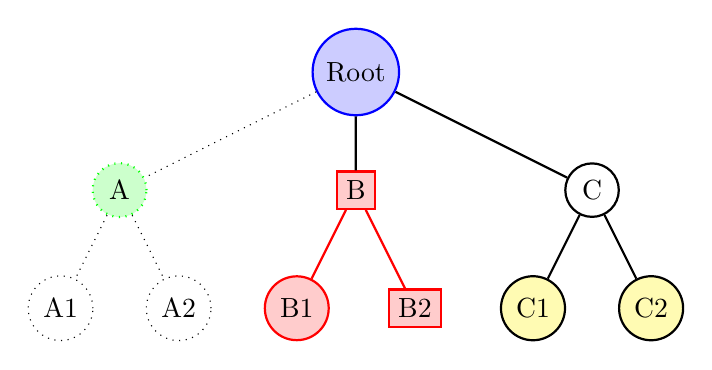
\begin{tikzpicture}[level/.style={sibling distance=3cm/#1}]
		\node[circle, draw, text=black, draw=blue, thick, fill=blue!20] {Root}
		child[dotted] { node[circle, draw, thick, text=black, draw=green, fill=green!20] {A}
				child {node[circle, draw] {A1}}
				child {node[circle, draw] {A2}}
			}
		child[thick] { node[rectangle, draw, text=black, draw=red, fill=red!20] {B}
				child[red] { node[circle, draw, text=black, fill=red!20] {B1}}
				child[red] { node[rectangle, draw, text=black, fill=red!20] {B2}}
			}
		child[thick] { node[circle, draw, text=black] {C}
				child { node[circle, draw, text=black, fill=yellow!30] {C1}}
				child { node[circle, draw, text=black, fill=yellow!30] {C2}}
			};
	\end{tikzpicture}
\end{center}

\begin{center}
	\begin{tikzpicture}[node distance=2cm, main node/.style={circle, draw, thick, font=\Large}]
		\node[main node, fill=green!20, draw=green, thick] (1) {1};
		\node[main node] (3) [below of=1] {3};
		\node[main node] (2) [right of=3] {2};
		\node[main node] (4) [left of=3] {4};
		\node[main node, fill=blue!20, draw=blue, thick] (5) [below of=3] {5};

		\path
		(1) edge[ultra thick, red] node[left, black] {1} (4)
		(1) edge[thick] node[left, black] {3} (3)
		(1) edge[thick] node[right, black] {2} (2)
		(3) edge[ultra thick, red] node[right, black] {2} (5)
		(3) edge[thick] node[above, black] {3} (2)
		(2) edge[thick] node[right, black] {4} (5)
		(3) edge[ultra thick, red] node[below, black] {1} (4)
		(4) edge[bend right, -Stealth, thick] (5);
	\end{tikzpicture}
\end{center}